\documentclass[1p]{elsarticle_modified}
%\bibliographystyle{elsarticle-num}

%\usepackage[colorlinks]{hyperref}
%\usepackage{abbrmath_seonhwa} %\Abb, \Ascr, \Acal ,\Abf, \Afrak
\usepackage{amsfonts}
\usepackage{amssymb}
\usepackage{amsmath}
\usepackage{amsthm}
\usepackage{scalefnt}
\usepackage{amsbsy}
\usepackage{kotex}
\usepackage{caption}
\usepackage{subfig}
\usepackage{color}
\usepackage{graphicx}
\usepackage{xcolor} %% white, black, red, green, blue, cyan, magenta, yellow
\usepackage{float}
\usepackage{setspace}
\usepackage{hyperref}

\usepackage{tikz}
\usetikzlibrary{arrows}

\usepackage{multirow}
\usepackage{array} % fixed length table
\usepackage{hhline}

%%%%%%%%%%%%%%%%%%%%%
\makeatletter
\renewcommand*\env@matrix[1][\arraystretch]{%
	\edef\arraystretch{#1}%
	\hskip -\arraycolsep
	\let\@ifnextchar\new@ifnextchar
	\array{*\c@MaxMatrixCols c}}
\makeatother %https://tex.stackexchange.com/questions/14071/how-can-i-increase-the-line-spacing-in-a-matrix
%%%%%%%%%%%%%%%

\usepackage[normalem]{ulem}

\newcommand{\msout}[1]{\ifmmode\text{\sout{\ensuremath{#1}}}\else\sout{#1}\fi}
%SOURCE: \msout is \stkout macro in https://tex.stackexchange.com/questions/20609/strikeout-in-math-mode

\newcommand{\cancel}[1]{
	\ifmmode
	{\color{red}\msout{#1}}
	\else
	{\color{red}\sout{#1}}
	\fi
}

\newcommand{\add}[1]{
	{\color{blue}\uwave{#1}}
}

\newcommand{\replace}[2]{
	\ifmmode
	{\color{red}\msout{#1}}{\color{blue}\uwave{#2}}
	\else
	{\color{red}\sout{#1}}{\color{blue}\uwave{#2}}
	\fi
}

\newcommand{\Sol}{\mathcal{S}} %segment
\newcommand{\D}{D} %diagram
\newcommand{\A}{\mathcal{A}} %arc


%%%%%%%%%%%%%%%%%%%%%%%%%%%%%5 test

\def\sl{\operatorname{\textup{SL}}(2,\Cbb)}
\def\psl{\operatorname{\textup{PSL}}(2,\Cbb)}
\def\quan{\mkern 1mu \triangleright \mkern 1mu}

\theoremstyle{definition}
\newtheorem{thm}{Theorem}[section]
\newtheorem{prop}[thm]{Proposition}
\newtheorem{lem}[thm]{Lemma}
\newtheorem{ques}[thm]{Question}
\newtheorem{cor}[thm]{Corollary}
\newtheorem{defn}[thm]{Definition}
\newtheorem{exam}[thm]{Example}
\newtheorem{rmk}[thm]{Remark}
\newtheorem{alg}[thm]{Algorithm}

\newcommand{\I}{\sqrt{-1}}
\begin{document}

%\begin{frontmatter}
%
%\title{Boundary parabolic representations of knots up to 8 crossings}
%
%%% Group authors per affiliation:
%\author{Yunhi Cho} 
%\address{Department of Mathematics, University of Seoul, Seoul, Korea}
%\ead{yhcho@uos.ac.kr}
%
%
%\author{Seonhwa Kim} %\fnref{s_kim}}
%\address{Center for Geometry and Physics, Institute for Basic Science, Pohang, 37673, Korea}
%\ead{ryeona17@ibs.re.kr}
%
%\author{Hyuk Kim}
%\address{Department of Mathematical Sciences, Seoul National University, Seoul 08826, Korea}
%\ead{hyukkim@snu.ac.kr}
%
%\author{Seokbeom Yoon}
%\address{Department of Mathematical Sciences, Seoul National University, Seoul, 08826,  Korea}
%\ead{sbyoon15@snu.ac.kr}
%
%\begin{abstract}
%We find all boundary parabolic representation of knots up to 8 crossings.
%
%\end{abstract}
%\begin{keyword}
%    \MSC[2010] 57M25 
%\end{keyword}
%
%\end{frontmatter}

%\linenumbers
%\tableofcontents
%
\newcommand\colored[1]{\textcolor{white}{\rule[-0.35ex]{0.8em}{1.4ex}}\kern-0.8em\color{red} #1}%
%\newcommand\colored[1]{\textcolor{white}{ #1}\kern-2.17ex	\textcolor{white}{ #1}\kern-1.81ex	\textcolor{white}{ #1}\kern-2.15ex\color{red}#1	}

{\Large $\underline{12a_{1015}~(K12a_{1015})}$}

\setlength{\tabcolsep}{10pt}
\renewcommand{\arraystretch}{1.6}
\vspace{1cm}\begin{tabular}{m{100pt}>{\centering\arraybackslash}m{274pt}}
\multirow{5}{120pt}{
	\centering
	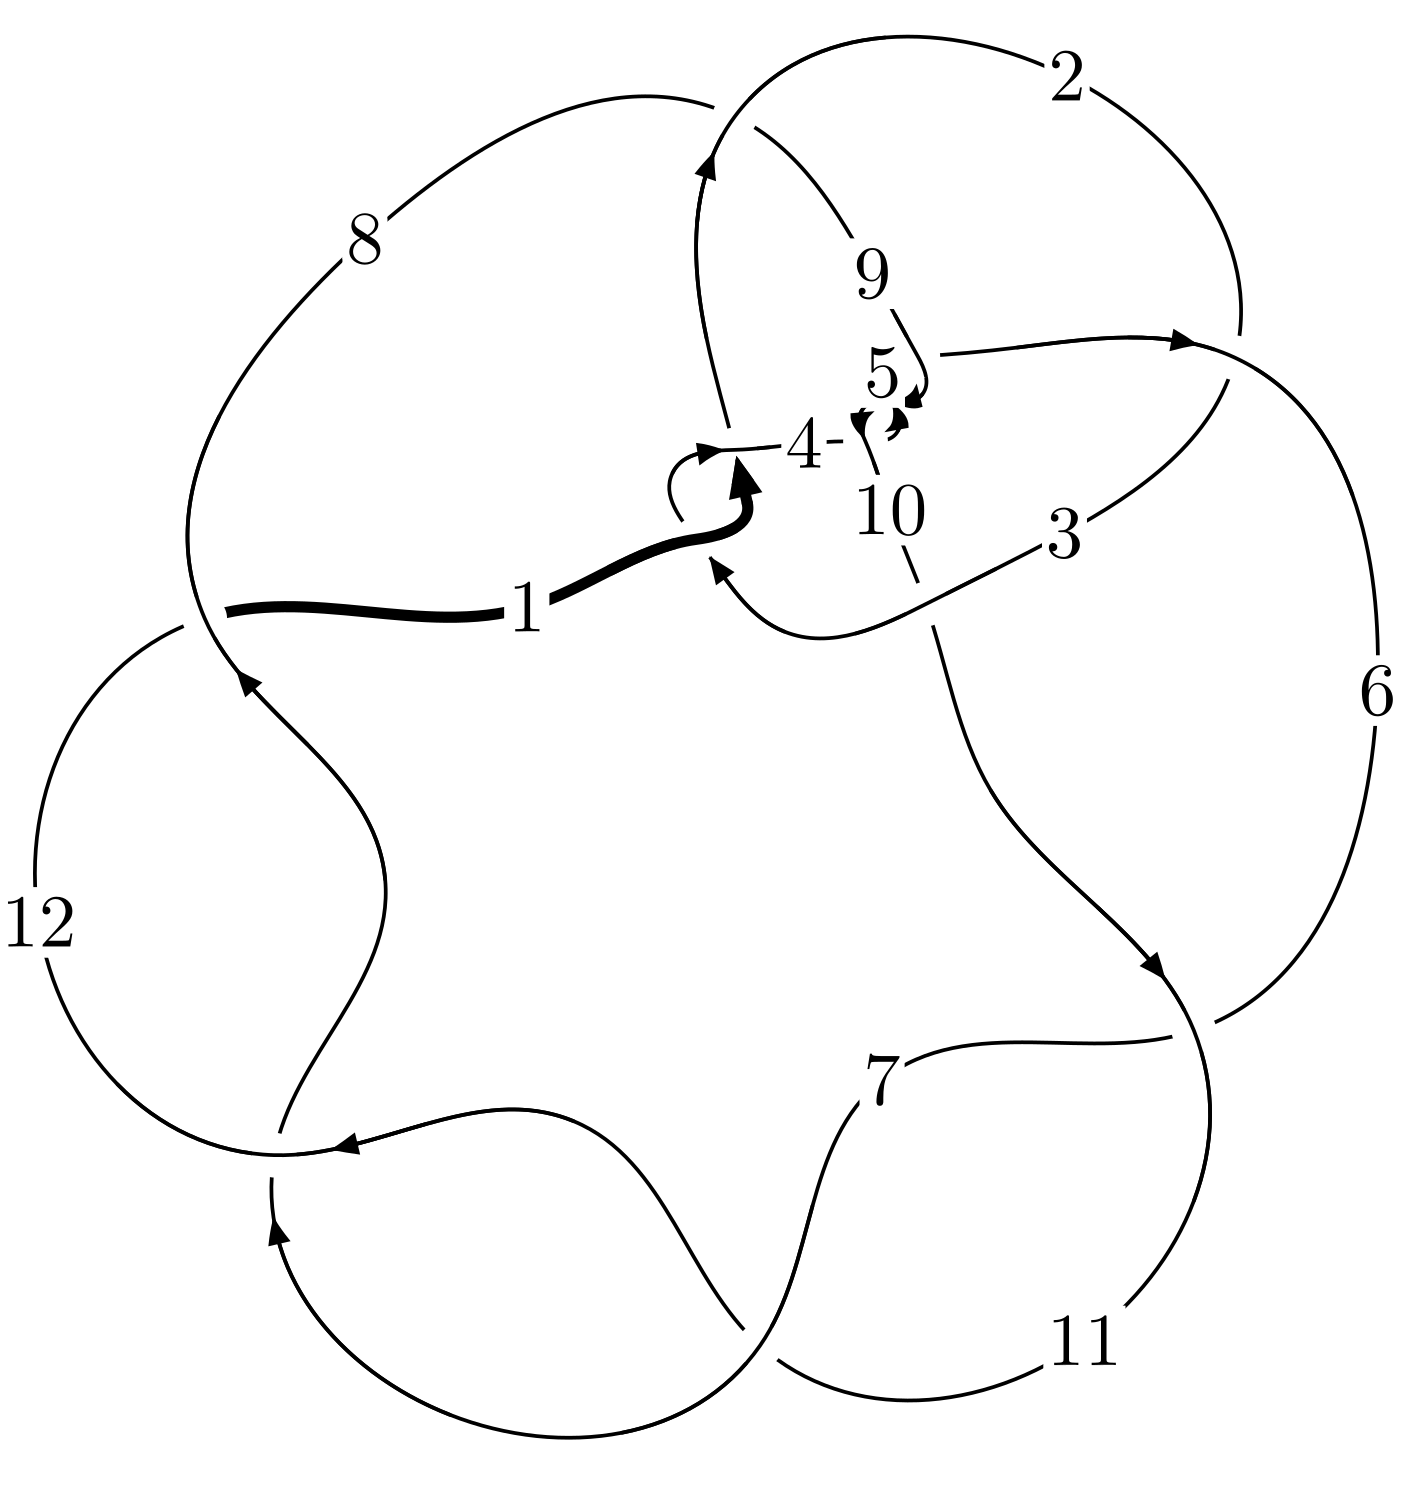
\includegraphics[width=112pt]{../../../GIT/diagram.site/Diagrams/png/1816_12a_1015.png}\\
\ \ \ A knot diagram\footnotemark}&
\allowdisplaybreaks
\textbf{Linearized knot diagam} \\
\cline{2-2}
 &
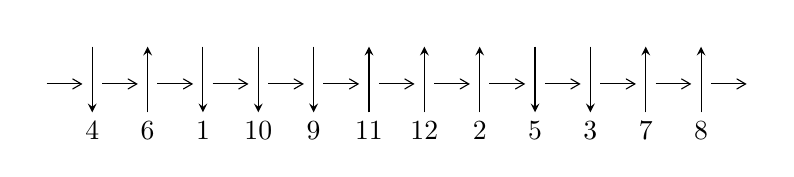
\begin{tikzpicture}[x=20pt, y=17pt]
	% nodes
	\node (C0) at (0, 0) {};
	\node (C1) at (1, 0) {};
	\node (C1U) at (1, +1) {};
	\node (C1D) at (1, -1) {4};

	\node (C2) at (2, 0) {};
	\node (C2U) at (2, +1) {};
	\node (C2D) at (2, -1) {6};

	\node (C3) at (3, 0) {};
	\node (C3U) at (3, +1) {};
	\node (C3D) at (3, -1) {1};

	\node (C4) at (4, 0) {};
	\node (C4U) at (4, +1) {};
	\node (C4D) at (4, -1) {10};

	\node (C5) at (5, 0) {};
	\node (C5U) at (5, +1) {};
	\node (C5D) at (5, -1) {9};

	\node (C6) at (6, 0) {};
	\node (C6U) at (6, +1) {};
	\node (C6D) at (6, -1) {11};

	\node (C7) at (7, 0) {};
	\node (C7U) at (7, +1) {};
	\node (C7D) at (7, -1) {12};

	\node (C8) at (8, 0) {};
	\node (C8U) at (8, +1) {};
	\node (C8D) at (8, -1) {2};

	\node (C9) at (9, 0) {};
	\node (C9U) at (9, +1) {};
	\node (C9D) at (9, -1) {5};

	\node (C10) at (10, 0) {};
	\node (C10U) at (10, +1) {};
	\node (C10D) at (10, -1) {3};

	\node (C11) at (11, 0) {};
	\node (C11U) at (11, +1) {};
	\node (C11D) at (11, -1) {7};

	\node (C12) at (12, 0) {};
	\node (C12U) at (12, +1) {};
	\node (C12D) at (12, -1) {8};
	\node (C13) at (13, 0) {};

	% arrows
	\draw[->,>={angle 60}]
	(C0) edge (C1) (C1) edge (C2) (C2) edge (C3) (C3) edge (C4) (C4) edge (C5) (C5) edge (C6) (C6) edge (C7) (C7) edge (C8) (C8) edge (C9) (C9) edge (C10) (C10) edge (C11) (C11) edge (C12) (C12) edge (C13) ;	\draw[->,>=stealth]
	(C1U) edge (C1D) (C2D) edge (C2U) (C3U) edge (C3D) (C4U) edge (C4D) (C5U) edge (C5D) (C6D) edge (C6U) (C7D) edge (C7U) (C8D) edge (C8U) (C9U) edge (C9D) (C10U) edge (C10D) (C11D) edge (C11U) (C12D) edge (C12U) ;
	\end{tikzpicture} \\
\hhline{~~} \\& 
\textbf{Solving Sequence} \\ \cline{2-2} 
 &
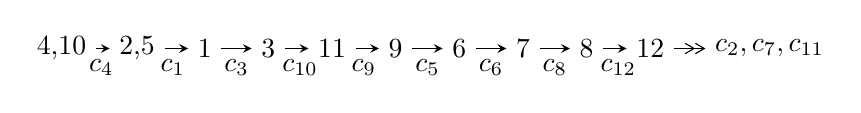
\begin{tikzpicture}[x=23pt, y=7pt]
	% node
	\node (A0) at (-1/8, 0) {4,10};
	\node (A1) at (17/16, 0) {2,5};
	\node (A2) at (17/8, 0) {1};
	\node (A3) at (25/8, 0) {3};
	\node (A4) at (33/8, 0) {11};
	\node (A5) at (41/8, 0) {9};
	\node (A6) at (49/8, 0) {6};
	\node (A7) at (57/8, 0) {7};
	\node (A8) at (65/8, 0) {8};
	\node (A9) at (73/8, 0) {12};
	\node (C1) at (1/2, -1) {$c_{4}$};
	\node (C2) at (13/8, -1) {$c_{1}$};
	\node (C3) at (21/8, -1) {$c_{3}$};
	\node (C4) at (29/8, -1) {$c_{10}$};
	\node (C5) at (37/8, -1) {$c_{9}$};
	\node (C6) at (45/8, -1) {$c_{5}$};
	\node (C7) at (53/8, -1) {$c_{6}$};
	\node (C8) at (61/8, -1) {$c_{8}$};
	\node (C9) at (69/8, -1) {$c_{12}$};
	\node (A10) at (11, 0) {$c_{2},c_{7},c_{11}$};

	% edge
	\draw[->,>=stealth]	
	(A0) edge (A1) (A1) edge (A2) (A2) edge (A3) (A3) edge (A4) (A4) edge (A5) (A5) edge (A6) (A6) edge (A7) (A7) edge (A8) (A8) edge (A9) ;
	\draw[->>,>={angle 60}]	
	(A9) edge (A10);
\end{tikzpicture} \\ 

\end{tabular} \\

\footnotetext{
The image of knot diagram is generated by the software ``\textbf{Draw programme}" developed by Andrew Bartholomew(\url{http://www.layer8.co.uk/maths/draw/index.htm\#Running-draw}), where we modified some parts for our purpose(\url{https://github.com/CATsTAILs/LinksPainter}).
}\phantom \\ \newline 
\centering \textbf{Ideals for irreducible components\footnotemark of $X_{\text{par}}$} 
 
\begin{align*}
I^u_{1}&=\langle 
6.55158\times10^{71} u^{69}-2.48630\times10^{71} u^{68}+\cdots+4.14466\times10^{73} b+4.49840\times10^{73},\\
\phantom{I^u_{1}}&\phantom{= \langle  }-5.30555\times10^{74} u^{69}-8.22334\times10^{74} u^{68}+\cdots+4.55913\times10^{74} a+1.52184\times10^{74},\;u^{70}+2 u^{69}+\cdots-2 u-1\rangle \\
I^u_{2}&=\langle 
b+1,\;6 u^4- u^3+4 u^2+11 a-6 u+2,\;u^5+u^4+2 u^3+u^2+u+1\rangle \\
\\
\end{align*}
\raggedright * 2 irreducible components of $\dim_{\mathbb{C}}=0$, with total 75 representations.\\
\footnotetext{All coefficients of polynomials are rational numbers. But the coefficients are sometimes approximated in decimal forms when there is not enough margin.}
\newpage
\renewcommand{\arraystretch}{1}
\centering \section*{I. $I^u_{1}= \langle 6.55\times10^{71} u^{69}-2.49\times10^{71} u^{68}+\cdots+4.14\times10^{73} b+4.50\times10^{73},\;-5.31\times10^{74} u^{69}-8.22\times10^{74} u^{68}+\cdots+4.56\times10^{74} a+1.52\times10^{74},\;u^{70}+2 u^{69}+\cdots-2 u-1 \rangle$}
\flushleft \textbf{(i) Arc colorings}\\
\begin{tabular}{m{7pt} m{180pt} m{7pt} m{180pt} }
\flushright $a_{4}=$&$\begin{pmatrix}1\\0\end{pmatrix}$ \\
\flushright $a_{10}=$&$\begin{pmatrix}0\\u\end{pmatrix}$ \\
\flushright $a_{2}=$&$\begin{pmatrix}1.16372 u^{69}+1.80371 u^{68}+\cdots-12.1418 u-0.333801\\-0.0158073 u^{69}+0.00599879 u^{68}+\cdots+0.128028 u-1.08535\end{pmatrix}$ \\
\flushright $a_{5}=$&$\begin{pmatrix}1\\u^2\end{pmatrix}$ \\
\flushright $a_{1}=$&$\begin{pmatrix}1.14791 u^{69}+1.80971 u^{68}+\cdots-12.0137 u-1.41915\\-0.0158073 u^{69}+0.00599879 u^{68}+\cdots+0.128028 u-1.08535\end{pmatrix}$ \\
\flushright $a_{3}=$&$\begin{pmatrix}1.16769 u^{69}+1.80098 u^{68}+\cdots-12.0610 u-0.269803\\0.0108796 u^{69}+0.0526221 u^{68}+\cdots+0.0867825 u-1.10387\end{pmatrix}$ \\
\flushright $a_{11}=$&$\begin{pmatrix}1.23789 u^{69}+2.97447 u^{68}+\cdots-8.93000 u-7.95394\\-0.537189 u^{69}-1.02248 u^{68}+\cdots+3.28194 u+1.05622\end{pmatrix}$ \\
\flushright $a_{9}=$&$\begin{pmatrix}u\\u^3+u\end{pmatrix}$ \\
\flushright $a_{6}=$&$\begin{pmatrix}u^2+1\\u^4+2 u^2\end{pmatrix}$ \\
\flushright $a_{7}=$&$\begin{pmatrix}-0.232208 u^{69}-0.851321 u^{68}+\cdots-2.00060 u+4.73175\\0.525839 u^{69}+0.960044 u^{68}+\cdots-1.03476 u-0.695269\end{pmatrix}$ \\
\flushright $a_{8}=$&$\begin{pmatrix}1.12189 u^{69}+2.81589 u^{68}+\cdots-3.33901 u-8.52558\\-0.674930 u^{69}-1.33241 u^{68}+\cdots+3.69661 u+1.16196\end{pmatrix}$ \\
\flushright $a_{12}=$&$\begin{pmatrix}1.19605 u^{69}+2.08859 u^{68}+\cdots-8.12152 u-5.32037\\-0.265234 u^{69}-0.371359 u^{68}+\cdots+1.22176 u-0.304010\end{pmatrix}$\\&\end{tabular}
\flushleft \textbf{(ii) Obstruction class $= -1$}\\~\\
\flushleft \textbf{(iii) Cusp Shapes $= 4.38477 u^{69}+8.26850 u^{68}+\cdots-26.9142 u-8.59413$}\\~\\
\newpage\renewcommand{\arraystretch}{1}
\flushleft \textbf{(iv) u-Polynomials at the component}\newline \\
\begin{tabular}{m{50pt}|m{274pt}}
Crossings & \hspace{64pt}u-Polynomials at each crossing \\
\hline $$\begin{aligned}c_{1},c_{3}\end{aligned}$$&$\begin{aligned}
&u^{70}-6 u^{69}+\cdots+1478 u-121
\end{aligned}$\\
\hline $$\begin{aligned}c_{2}\end{aligned}$$&$\begin{aligned}
&u^{70}-5 u^{69}+\cdots-29568 u+3872
\end{aligned}$\\
\hline $$\begin{aligned}c_{4},c_{5},c_{9}\end{aligned}$$&$\begin{aligned}
&u^{70}+2 u^{69}+\cdots-2 u-1
\end{aligned}$\\
\hline $$\begin{aligned}c_{6},c_{7},c_{11}\\c_{12}\end{aligned}$$&$\begin{aligned}
&u^{70}+2 u^{69}+\cdots-2 u+1
\end{aligned}$\\
\hline $$\begin{aligned}c_{8}\end{aligned}$$&$\begin{aligned}
&11(11 u^{70}-25 u^{69}+\cdots-132109 u-43949)
\end{aligned}$\\
\hline $$\begin{aligned}c_{10}\end{aligned}$$&$\begin{aligned}
&11(11 u^{70}-8 u^{69}+\cdots+29588 u+17257)
\end{aligned}$\\
\hline
\end{tabular}\\~\\
\newpage\renewcommand{\arraystretch}{1}
\flushleft \textbf{(v) Riley Polynomials at the component}\newline \\
\begin{tabular}{m{50pt}|m{274pt}}
Crossings & \hspace{64pt}Riley Polynomials at each crossing \\
\hline $$\begin{aligned}c_{1},c_{3}\end{aligned}$$&$\begin{aligned}
&y^{70}-34 y^{69}+\cdots-90458 y+14641
\end{aligned}$\\
\hline $$\begin{aligned}c_{2}\end{aligned}$$&$\begin{aligned}
&y^{70}-33 y^{69}+\cdots-229160448 y+14992384
\end{aligned}$\\
\hline $$\begin{aligned}c_{4},c_{5},c_{9}\end{aligned}$$&$\begin{aligned}
&y^{70}+66 y^{69}+\cdots-4 y+1
\end{aligned}$\\
\hline $$\begin{aligned}c_{6},c_{7},c_{11}\\c_{12}\end{aligned}$$&$\begin{aligned}
&y^{70}-82 y^{69}+\cdots-4 y+1
\end{aligned}$\\
\hline $$\begin{aligned}c_{8}\end{aligned}$$&$\begin{aligned}
&121(121 y^{70}-3045 y^{69}+\cdots-4.12871\times10^{10} y+1.93151\times10^{9})
\end{aligned}$\\
\hline $$\begin{aligned}c_{10}\end{aligned}$$&$\begin{aligned}
&121(121 y^{70}+4358 y^{69}+\cdots+3.69634\times10^{9} y+2.97804\times10^{8})
\end{aligned}$\\
\hline
\end{tabular}\\~\\
\newpage\flushleft \textbf{(vi) Complex Volumes and Cusp Shapes}
$$\begin{array}{c|c|c}  
\text{Solutions to }I^u_{1}& \I (\text{vol} + \sqrt{-1}CS) & \text{Cusp shape}\\
 \hline 
\begin{aligned}
u &= \phantom{-}0.686400 + 0.713366 I \\
a &= -0.053948 - 0.210944 I \\
b &= \phantom{-}0.951229 - 0.454660 I\end{aligned}
 & \phantom{-}0.87667 + 3.35580 I & \phantom{-0.000000 } 0 \\ \hline\begin{aligned}
u &= \phantom{-}0.686400 - 0.713366 I \\
a &= -0.053948 + 0.210944 I \\
b &= \phantom{-}0.951229 + 0.454660 I\end{aligned}
 & \phantom{-}0.87667 - 3.35580 I & \phantom{-0.000000 } 0 \\ \hline\begin{aligned}
u &= -0.713932 + 0.648184 I \\
a &= -0.188351 + 0.239557 I \\
b &= \phantom{-}1.094430 + 0.592356 I\end{aligned}
 & \phantom{-}8.96389 - 6.20258 I & \phantom{-0.000000 } 0 \\ \hline\begin{aligned}
u &= -0.713932 - 0.648184 I \\
a &= -0.188351 - 0.239557 I \\
b &= \phantom{-}1.094430 - 0.592356 I\end{aligned}
 & \phantom{-}8.96389 + 6.20258 I & \phantom{-0.000000 } 0 \\ \hline\begin{aligned}
u &= -0.597225 + 0.868784 I \\
a &= \phantom{-}0.131337 + 0.213010 I \\
b &= \phantom{-}0.779698 + 0.239595 I\end{aligned}
 & -0.594033 + 1.028690 I & \phantom{-0.000000 } 0 \\ \hline\begin{aligned}
u &= -0.597225 - 0.868784 I \\
a &= \phantom{-}0.131337 - 0.213010 I \\
b &= \phantom{-}0.779698 - 0.239595 I\end{aligned}
 & -0.594033 - 1.028690 I & \phantom{-0.000000 } 0 \\ \hline\begin{aligned}
u &= -0.844565 + 0.393225 I \\
a &= \phantom{-}0.756345 + 0.697914 I \\
b &= \phantom{-}1.027460 - 0.439585 I\end{aligned}
 & -1.98877 + 4.08537 I & \phantom{-0.000000 } 0. - 6.03382 I \\ \hline\begin{aligned}
u &= -0.844565 - 0.393225 I \\
a &= \phantom{-}0.756345 - 0.697914 I \\
b &= \phantom{-}1.027460 + 0.439585 I\end{aligned}
 & -1.98877 - 4.08537 I & \phantom{-0.000000 -}0. + 6.03382 I \\ \hline\begin{aligned}
u &= \phantom{-}0.816696 + 0.440810 I \\
a &= \phantom{-}0.730245 - 0.900336 I \\
b &= \phantom{-}1.155090 + 0.559766 I\end{aligned}
 & \phantom{-}0.05014 - 8.48498 I & \phantom{-0.000000 -}0. + 9.02977 I \\ \hline\begin{aligned}
u &= \phantom{-}0.816696 - 0.440810 I \\
a &= \phantom{-}0.730245 + 0.900336 I \\
b &= \phantom{-}1.155090 - 0.559766 I\end{aligned}
 & \phantom{-}0.05014 + 8.48498 I & \phantom{-0.000000 } 0. - 9.02977 I\\
 \hline 
 \end{array}$$\newpage$$\begin{array}{c|c|c}  
\text{Solutions to }I^u_{1}& \I (\text{vol} + \sqrt{-1}CS) & \text{Cusp shape}\\
 \hline 
\begin{aligned}
u &= -0.797710 + 0.463395 I \\
a &= \phantom{-}0.733935 + 1.050130 I \\
b &= \phantom{-}1.238960 - 0.666041 I\end{aligned}
 & \phantom{-}8.39434 + 11.28920 I & \phantom{-0.000000 } 0. - 7.45273 I \\ \hline\begin{aligned}
u &= -0.797710 - 0.463395 I \\
a &= \phantom{-}0.733935 - 1.050130 I \\
b &= \phantom{-}1.238960 + 0.666041 I\end{aligned}
 & \phantom{-}8.39434 - 11.28920 I & \phantom{-0.000000 -}0. + 7.45273 I \\ \hline\begin{aligned}
u &= \phantom{-}0.794883 + 0.243299 I \\
a &= \phantom{-}0.990789 - 0.382417 I \\
b &= \phantom{-}0.722317 + 0.329197 I\end{aligned}
 & \phantom{-}1.74452 - 0.22556 I & \phantom{-}6.21604 + 2.91678 I \\ \hline\begin{aligned}
u &= \phantom{-}0.794883 - 0.243299 I \\
a &= \phantom{-}0.990789 + 0.382417 I \\
b &= \phantom{-}0.722317 - 0.329197 I\end{aligned}
 & \phantom{-}1.74452 + 0.22556 I & \phantom{-}6.21604 - 2.91678 I \\ \hline\begin{aligned}
u &= -0.578794 + 0.475444 I \\
a &= -0.214985 - 0.392745 I \\
b &= \phantom{-}0.298756 + 1.109540 I\end{aligned}
 & \phantom{-}11.29930 + 5.03905 I & \phantom{-}6.42974 - 5.21383 I \\ \hline\begin{aligned}
u &= -0.578794 - 0.475444 I \\
a &= -0.214985 + 0.392745 I \\
b &= \phantom{-}0.298756 - 1.109540 I\end{aligned}
 & \phantom{-}11.29930 - 5.03905 I & \phantom{-}6.42974 + 5.21383 I \\ \hline\begin{aligned}
u &= -0.077426 + 1.268050 I \\
a &= \phantom{-}1.26161 - 1.02736 I \\
b &= -1.67281 + 0.43951 I\end{aligned}
 & \phantom{-}7.81603 + 2.12622 I & \phantom{-0.000000 } 0 \\ \hline\begin{aligned}
u &= -0.077426 - 1.268050 I \\
a &= \phantom{-}1.26161 + 1.02736 I \\
b &= -1.67281 - 0.43951 I\end{aligned}
 & \phantom{-}7.81603 - 2.12622 I & \phantom{-0.000000 } 0 \\ \hline\begin{aligned}
u &= -0.631247 + 0.350474 I \\
a &= \phantom{-}1.50034 + 0.57008 I \\
b &= \phantom{-}0.428001 - 0.725712 I\end{aligned}
 & \phantom{-}10.93100 - 1.15018 I & \phantom{-}6.37418 - 2.37950 I \\ \hline\begin{aligned}
u &= -0.631247 - 0.350474 I \\
a &= \phantom{-}1.50034 - 0.57008 I \\
b &= \phantom{-}0.428001 + 0.725712 I\end{aligned}
 & \phantom{-}10.93100 + 1.15018 I & \phantom{-}6.37418 + 2.37950 I\\
 \hline 
 \end{array}$$\newpage$$\begin{array}{c|c|c}  
\text{Solutions to }I^u_{1}& \I (\text{vol} + \sqrt{-1}CS) & \text{Cusp shape}\\
 \hline 
\begin{aligned}
u &= \phantom{-}0.514246 + 1.178650 I \\
a &= \phantom{-}0.234389 - 0.422329 I \\
b &= \phantom{-}0.777133 + 0.038992 I\end{aligned}
 & \phantom{-}4.70260 - 4.51481 I & \phantom{-0.000000 } 0 \\ \hline\begin{aligned}
u &= \phantom{-}0.514246 - 1.178650 I \\
a &= \phantom{-}0.234389 + 0.422329 I \\
b &= \phantom{-}0.777133 - 0.038992 I\end{aligned}
 & \phantom{-}4.70260 + 4.51481 I & \phantom{-0.000000 } 0 \\ \hline\begin{aligned}
u &= \phantom{-}0.514025 + 0.489099 I \\
a &= -0.032586 + 0.387308 I \\
b &= \phantom{-}0.207073 - 0.842044 I\end{aligned}
 & \phantom{-}2.79286 - 3.41411 I & \phantom{-}6.06553 + 7.18074 I \\ \hline\begin{aligned}
u &= \phantom{-}0.514025 - 0.489099 I \\
a &= -0.032586 - 0.387308 I \\
b &= \phantom{-}0.207073 + 0.842044 I\end{aligned}
 & \phantom{-}2.79286 + 3.41411 I & \phantom{-}6.06553 - 7.18074 I \\ \hline\begin{aligned}
u &= \phantom{-}0.027572 + 1.293330 I \\
a &= \phantom{-}0.713439 + 0.469428 I \\
b &= -1.50053 - 0.15574 I\end{aligned}
 & \phantom{-}1.11976 - 1.25245 I & \phantom{-0.000000 } 0 \\ \hline\begin{aligned}
u &= \phantom{-}0.027572 - 1.293330 I \\
a &= \phantom{-}0.713439 - 0.469428 I \\
b &= -1.50053 + 0.15574 I\end{aligned}
 & \phantom{-}1.11976 + 1.25245 I & \phantom{-0.000000 } 0 \\ \hline\begin{aligned}
u &= \phantom{-}0.094528 + 1.350430 I \\
a &= \phantom{-}0.61333 + 1.65329 I \\
b &= -1.103700 - 0.576201 I\end{aligned}
 & \phantom{-}2.07680 - 1.88125 I & \phantom{-0.000000 } 0 \\ \hline\begin{aligned}
u &= \phantom{-}0.094528 - 1.350430 I \\
a &= \phantom{-}0.61333 - 1.65329 I \\
b &= -1.103700 + 0.576201 I\end{aligned}
 & \phantom{-}2.07680 + 1.88125 I & \phantom{-0.000000 } 0 \\ \hline\begin{aligned}
u &= -0.133575 + 1.362630 I \\
a &= \phantom{-}0.64422 - 1.85435 I \\
b &= -0.974789 + 0.908157 I\end{aligned}
 & \phantom{-}3.26167 + 4.51191 I & \phantom{-0.000000 } 0 \\ \hline\begin{aligned}
u &= -0.133575 - 1.362630 I \\
a &= \phantom{-}0.64422 + 1.85435 I \\
b &= -0.974789 - 0.908157 I\end{aligned}
 & \phantom{-}3.26167 - 4.51191 I & \phantom{-0.000000 } 0\\
 \hline 
 \end{array}$$\newpage$$\begin{array}{c|c|c}  
\text{Solutions to }I^u_{1}& \I (\text{vol} + \sqrt{-1}CS) & \text{Cusp shape}\\
 \hline 
\begin{aligned}
u &= \phantom{-}0.161960 + 1.367850 I \\
a &= \phantom{-}0.56308 + 2.05596 I \\
b &= -0.91957 - 1.18906 I\end{aligned}
 & \phantom{-}10.78790 - 5.95071 I & \phantom{-0.000000 } 0 \\ \hline\begin{aligned}
u &= \phantom{-}0.161960 - 1.367850 I \\
a &= \phantom{-}0.56308 - 2.05596 I \\
b &= -0.91957 + 1.18906 I\end{aligned}
 & \phantom{-}10.78790 + 5.95071 I & \phantom{-0.000000 } 0 \\ \hline\begin{aligned}
u &= -0.057325 + 1.397340 I \\
a &= \phantom{-}0.79387 - 2.50536 I \\
b &= -0.854433 + 0.178775 I\end{aligned}
 & \phantom{-}4.63360 + 0.45945 I & \phantom{-0.000000 } 0 \\ \hline\begin{aligned}
u &= -0.057325 - 1.397340 I \\
a &= \phantom{-}0.79387 + 2.50536 I \\
b &= -0.854433 - 0.178775 I\end{aligned}
 & \phantom{-}4.63360 - 0.45945 I & \phantom{-0.000000 } 0 \\ \hline\begin{aligned}
u &= \phantom{-}0.05431 + 1.42323 I \\
a &= \phantom{-}2.44209 + 2.39720 I \\
b &= -0.772974 + 0.037973 I\end{aligned}
 & \phantom{-}12.68320 + 0.08405 I & \phantom{-0.000000 } 0 \\ \hline\begin{aligned}
u &= \phantom{-}0.05431 - 1.42323 I \\
a &= \phantom{-}2.44209 - 2.39720 I \\
b &= -0.772974 - 0.037973 I\end{aligned}
 & \phantom{-}12.68320 - 0.08405 I & \phantom{-0.000000 } 0 \\ \hline\begin{aligned}
u &= \phantom{-}0.575705\phantom{ +0.000000I} \\
a &= \phantom{-}1.22607\phantom{ +0.000000I} \\
b &= \phantom{-}0.312657\phantom{ +0.000000I}\end{aligned}
 & \phantom{-}1.70984\phantom{ +0.000000I} & \phantom{-}5.97300\phantom{ +0.000000I} \\ \hline\begin{aligned}
u &= \phantom{-}0.522828 + 0.213932 I \\
a &= -0.301618 + 0.925186 I \\
b &= -1.078510 - 0.834623 I\end{aligned}
 & \phantom{-}5.80188 - 3.48693 I & \phantom{-}0.21256 + 6.26702 I \\ \hline\begin{aligned}
u &= \phantom{-}0.522828 - 0.213932 I \\
a &= -0.301618 - 0.925186 I \\
b &= -1.078510 + 0.834623 I\end{aligned}
 & \phantom{-}5.80188 + 3.48693 I & \phantom{-}0.21256 - 6.26702 I \\ \hline\begin{aligned}
u &= -0.27390 + 1.43660 I \\
a &= \phantom{-}0.53012 + 1.40501 I \\
b &= \phantom{-}0.798447 - 0.686186 I\end{aligned}
 & \phantom{-}16.5894 + 2.2326 I & \phantom{-0.000000 } 0\\
 \hline 
 \end{array}$$\newpage$$\begin{array}{c|c|c}  
\text{Solutions to }I^u_{1}& \I (\text{vol} + \sqrt{-1}CS) & \text{Cusp shape}\\
 \hline 
\begin{aligned}
u &= -0.27390 - 1.43660 I \\
a &= \phantom{-}0.53012 - 1.40501 I \\
b &= \phantom{-}0.798447 + 0.686186 I\end{aligned}
 & \phantom{-}16.5894 - 2.2326 I & \phantom{-0.000000 } 0 \\ \hline\begin{aligned}
u &= -0.296415 + 0.442080 I \\
a &= \phantom{-}0.505486 - 0.384301 I \\
b &= \phantom{-}0.011825 + 0.286358 I\end{aligned}
 & \phantom{-}0.074574 + 0.954323 I & \phantom{-}1.69242 - 6.62051 I \\ \hline\begin{aligned}
u &= -0.296415 - 0.442080 I \\
a &= \phantom{-}0.505486 + 0.384301 I \\
b &= \phantom{-}0.011825 - 0.286358 I\end{aligned}
 & \phantom{-}0.074574 - 0.954323 I & \phantom{-}1.69242 + 6.62051 I \\ \hline\begin{aligned}
u &= -0.516350\phantom{ +0.000000I} \\
a &= -0.747230\phantom{ +0.000000I} \\
b &= -1.59427\phantom{ +0.000000I}\end{aligned}
 & \phantom{-}4.13003\phantom{ +0.000000I} & -2.66790\phantom{ +0.000000I} \\ \hline\begin{aligned}
u &= \phantom{-}0.31116 + 1.45838 I \\
a &= \phantom{-}0.165497 - 1.346330 I \\
b &= \phantom{-}0.987560 + 0.582127 I\end{aligned}
 & \phantom{-}7.32955 - 4.26678 I & \phantom{-0.000000 } 0 \\ \hline\begin{aligned}
u &= \phantom{-}0.31116 - 1.45838 I \\
a &= \phantom{-}0.165497 + 1.346330 I \\
b &= \phantom{-}0.987560 - 0.582127 I\end{aligned}
 & \phantom{-}7.32955 + 4.26678 I & \phantom{-0.000000 } 0 \\ \hline\begin{aligned}
u &= \phantom{-}0.18529 + 1.48231 I \\
a &= -0.56128 + 1.40862 I \\
b &= \phantom{-}0.350564 - 1.174690 I\end{aligned}
 & \phantom{-}9.18672 - 6.01404 I & \phantom{-0.000000 } 0 \\ \hline\begin{aligned}
u &= \phantom{-}0.18529 - 1.48231 I \\
a &= -0.56128 - 1.40862 I \\
b &= \phantom{-}0.350564 + 1.174690 I\end{aligned}
 & \phantom{-}9.18672 + 6.01404 I & \phantom{-0.000000 } 0 \\ \hline\begin{aligned}
u &= -0.20329 + 1.48122 I \\
a &= -0.76720 - 1.54412 I \\
b &= \phantom{-}0.44380 + 1.35657 I\end{aligned}
 & \phantom{-}17.6404 + 7.9075 I & \phantom{-0.000000 } 0 \\ \hline\begin{aligned}
u &= -0.20329 - 1.48122 I \\
a &= -0.76720 + 1.54412 I \\
b &= \phantom{-}0.44380 - 1.35657 I\end{aligned}
 & \phantom{-}17.6404 - 7.9075 I & \phantom{-0.000000 } 0\\
 \hline 
 \end{array}$$\newpage$$\begin{array}{c|c|c}  
\text{Solutions to }I^u_{1}& \I (\text{vol} + \sqrt{-1}CS) & \text{Cusp shape}\\
 \hline 
\begin{aligned}
u &= -0.465530 + 0.181096 I \\
a &= -0.482595 - 1.101610 I \\
b &= -1.074710 + 0.528711 I\end{aligned}
 & -1.59167 + 2.36731 I & -3.11903 - 9.00869 I \\ \hline\begin{aligned}
u &= -0.465530 - 0.181096 I \\
a &= -0.482595 + 1.101610 I \\
b &= -1.074710 - 0.528711 I\end{aligned}
 & -1.59167 - 2.36731 I & -3.11903 + 9.00869 I \\ \hline\begin{aligned}
u &= -0.15387 + 1.49344 I \\
a &= -0.313268 - 1.110630 I \\
b &= \phantom{-}0.304389 + 0.861897 I\end{aligned}
 & \phantom{-}6.62342 + 2.84491 I & \phantom{-0.000000 } 0 \\ \hline\begin{aligned}
u &= -0.15387 - 1.49344 I \\
a &= -0.313268 + 1.110630 I \\
b &= \phantom{-}0.304389 - 0.861897 I\end{aligned}
 & \phantom{-}6.62342 - 2.84491 I & \phantom{-0.000000 } 0 \\ \hline\begin{aligned}
u &= -0.31045 + 1.49001 I \\
a &= -0.09717 + 1.48789 I \\
b &= \phantom{-}1.160460 - 0.608170 I\end{aligned}
 & \phantom{-}4.10310 + 8.26194 I & \phantom{-0.000000 } 0 \\ \hline\begin{aligned}
u &= -0.31045 - 1.49001 I \\
a &= -0.09717 - 1.48789 I \\
b &= \phantom{-}1.160460 + 0.608170 I\end{aligned}
 & \phantom{-}4.10310 - 8.26194 I & \phantom{-0.000000 } 0 \\ \hline\begin{aligned}
u &= \phantom{-}0.212174 + 0.423840 I \\
a &= \phantom{-}3.71972 + 1.14676 I \\
b &= -1.020370 + 0.337236 I\end{aligned}
 & \phantom{-}6.92279 + 1.01855 I & \phantom{-}7.26660 + 6.17697 I \\ \hline\begin{aligned}
u &= \phantom{-}0.212174 - 0.423840 I \\
a &= \phantom{-}3.71972 - 1.14676 I \\
b &= -1.020370 - 0.337236 I\end{aligned}
 & \phantom{-}6.92279 - 1.01855 I & \phantom{-}7.26660 - 6.17697 I \\ \hline\begin{aligned}
u &= \phantom{-}0.29881 + 1.50168 I \\
a &= -0.19283 - 1.67138 I \\
b &= \phantom{-}1.25053 + 0.69071 I\end{aligned}
 & \phantom{-}6.33511 - 12.54100 I & \phantom{-0.000000 } 0 \\ \hline\begin{aligned}
u &= \phantom{-}0.29881 - 1.50168 I \\
a &= -0.19283 + 1.67138 I \\
b &= \phantom{-}1.25053 - 0.69071 I\end{aligned}
 & \phantom{-}6.33511 + 12.54100 I & \phantom{-0.000000 } 0\\
 \hline 
 \end{array}$$\newpage$$\begin{array}{c|c|c}  
\text{Solutions to }I^u_{1}& \I (\text{vol} + \sqrt{-1}CS) & \text{Cusp shape}\\
 \hline 
\begin{aligned}
u &= -0.29039 + 1.50769 I \\
a &= -0.24071 + 1.82752 I \\
b &= \phantom{-}1.30886 - 0.76850 I\end{aligned}
 & \phantom{-}14.7792 + 15.2576 I & \phantom{-0.000000 } 0 \\ \hline\begin{aligned}
u &= -0.29039 - 1.50769 I \\
a &= -0.24071 - 1.82752 I \\
b &= \phantom{-}1.30886 + 0.76850 I\end{aligned}
 & \phantom{-}14.7792 - 15.2576 I & \phantom{-0.000000 } 0 \\ \hline\begin{aligned}
u &= \phantom{-}0.15367 + 1.54248 I \\
a &= -0.510964 + 0.695006 I \\
b &= \phantom{-}0.606981 - 0.660450 I\end{aligned}
 & \phantom{-}8.47071 + 0.57802 I & \phantom{-0.000000 } 0 \\ \hline\begin{aligned}
u &= \phantom{-}0.15367 - 1.54248 I \\
a &= -0.510964 - 0.695006 I \\
b &= \phantom{-}0.606981 + 0.660450 I\end{aligned}
 & \phantom{-}8.47071 - 0.57802 I & \phantom{-0.000000 } 0 \\ \hline\begin{aligned}
u &= -0.18664 + 1.56544 I \\
a &= -0.799854 - 0.540948 I \\
b &= \phantom{-}0.866770 + 0.671583 I\end{aligned}
 & \phantom{-}16.3833 - 2.9707 I & \phantom{-0.000000 } 0 \\ \hline\begin{aligned}
u &= -0.18664 - 1.56544 I \\
a &= -0.799854 + 0.540948 I \\
b &= \phantom{-}0.866770 - 0.671583 I\end{aligned}
 & \phantom{-}16.3833 + 2.9707 I & \phantom{-0.000000 } 0 \\ \hline\begin{aligned}
u &= \phantom{-}0.410685 + 0.072099 I \\
a &= -1.48188 + 0.86518 I \\
b &= -1.199220 - 0.163900 I\end{aligned}
 & -2.39243 - 0.16622 I & -6.14498 - 3.46672 I \\ \hline\begin{aligned}
u &= \phantom{-}0.410685 - 0.072099 I \\
a &= -1.48188 - 0.86518 I \\
b &= -1.199220 + 0.163900 I\end{aligned}
 & -2.39243 + 0.16622 I & -6.14498 + 3.46672 I \\ \hline\begin{aligned}
u &= -0.176628 + 0.303504 I \\
a &= \phantom{-}4.01544 - 3.09185 I \\
b &= -0.957887 - 0.108785 I\end{aligned}
 & -0.643301 - 0.452052 I & \phantom{-}0.8141 - 14.9412 I \\ \hline\begin{aligned}
u &= -0.176628 - 0.303504 I \\
a &= \phantom{-}4.01544 + 3.09185 I \\
b &= -0.957887 + 0.108785 I\end{aligned}
 & -0.643301 + 0.452052 I & \phantom{-}0.8141 + 14.9412 I\\
 \hline 
 \end{array}$$\newpage\newpage\renewcommand{\arraystretch}{1}
\centering \section*{II. $I^u_{2}= \langle b+1,\;6 u^4- u^3+4 u^2+11 a-6 u+2,\;u^5+u^4+2 u^3+u^2+u+1 \rangle$}
\flushleft \textbf{(i) Arc colorings}\\
\begin{tabular}{m{7pt} m{180pt} m{7pt} m{180pt} }
\flushright $a_{4}=$&$\begin{pmatrix}1\\0\end{pmatrix}$ \\
\flushright $a_{10}=$&$\begin{pmatrix}0\\u\end{pmatrix}$ \\
\flushright $a_{2}=$&$\begin{pmatrix}-0.545455 u^{4}+0.0909091 u^{3}+\cdots+0.545455 u-0.181818\\-1\end{pmatrix}$ \\
\flushright $a_{5}=$&$\begin{pmatrix}1\\u^2\end{pmatrix}$ \\
\flushright $a_{1}=$&$\begin{pmatrix}-0.545455 u^{4}+0.0909091 u^{3}+\cdots+0.545455 u-1.18182\\-1\end{pmatrix}$ \\
\flushright $a_{3}=$&$\begin{pmatrix}-0.545455 u^{4}+0.0909091 u^{3}+\cdots+0.545455 u-0.181818\\-1\end{pmatrix}$ \\
\flushright $a_{11}=$&$\begin{pmatrix}0.280992 u^{4}-0.0165289 u^{3}+\cdots+0.0826446 u+0.487603\\0.636364 u^{4}+0.727273 u^{3}+\cdots+1.36364 u+0.545455\end{pmatrix}$ \\
\flushright $a_{9}=$&$\begin{pmatrix}u\\u^3+u\end{pmatrix}$ \\
\flushright $a_{6}=$&$\begin{pmatrix}u^2+1\\u^4+2 u^2\end{pmatrix}$ \\
\flushright $a_{7}=$&$\begin{pmatrix}0.157025 u^{4}+0.0495868 u^{3}+\cdots-0.247934 u+1.53719\\0.0909091 u^{4}-0.181818 u^{3}+\cdots-0.0909091 u+0.363636\end{pmatrix}$ \\
\flushright $a_{8}=$&$\begin{pmatrix}-0.0991736 u^{4}-0.347107 u^{3}+\cdots+0.735537 u+0.239669\\0.363636 u^{4}+1.27273 u^{3}+\cdots+1.63636 u+0.454545\end{pmatrix}$ \\
\flushright $a_{12}=$&$\begin{pmatrix}-1.24793 u^{4}+0.132231 u^{3}+\cdots+0.338843 u-0.900826\\-1.09091 u^{4}-0.818182 u^{3}+\cdots+0.0909091 u-1.36364\end{pmatrix}$\\&\end{tabular}
\flushleft \textbf{(ii) Obstruction class $= 1$}\\~\\
\flushleft \textbf{(iii) Cusp Shapes $= -\frac{4}{121} u^4+\frac{349}{121} u^3+\frac{441}{121} u^2+\frac{554}{121} u-\frac{71}{121}$}\\~\\
\newpage\renewcommand{\arraystretch}{1}
\flushleft \textbf{(iv) u-Polynomials at the component}\newline \\
\begin{tabular}{m{50pt}|m{274pt}}
Crossings & \hspace{64pt}u-Polynomials at each crossing \\
\hline $$\begin{aligned}c_{1}\end{aligned}$$&$\begin{aligned}
&(u-1)^5
\end{aligned}$\\
\hline $$\begin{aligned}c_{2}\end{aligned}$$&$\begin{aligned}
&u^5
\end{aligned}$\\
\hline $$\begin{aligned}c_{3}\end{aligned}$$&$\begin{aligned}
&(u+1)^5
\end{aligned}$\\
\hline $$\begin{aligned}c_{4},c_{5}\end{aligned}$$&$\begin{aligned}
&u^5+u^4+2 u^3+u^2+u+1
\end{aligned}$\\
\hline $$\begin{aligned}c_{6},c_{7}\end{aligned}$$&$\begin{aligned}
&u^5- u^4-2 u^3+u^2+u+1
\end{aligned}$\\
\hline $$\begin{aligned}c_{8}\end{aligned}$$&$\begin{aligned}
&11(11 u^5-2 u^4+6 u^3+u^2+1)
\end{aligned}$\\
\hline $$\begin{aligned}c_{9}\end{aligned}$$&$\begin{aligned}
&u^5- u^4+2 u^3- u^2+u-1
\end{aligned}$\\
\hline $$\begin{aligned}c_{10}\end{aligned}$$&$\begin{aligned}
&11(11 u^5+13 u^4-3 u^2+u+1)
\end{aligned}$\\
\hline $$\begin{aligned}c_{11},c_{12}\end{aligned}$$&$\begin{aligned}
&u^5+u^4-2 u^3- u^2+u-1
\end{aligned}$\\
\hline
\end{tabular}\\~\\
\newpage\renewcommand{\arraystretch}{1}
\flushleft \textbf{(v) Riley Polynomials at the component}\newline \\
\begin{tabular}{m{50pt}|m{274pt}}
Crossings & \hspace{64pt}Riley Polynomials at each crossing \\
\hline $$\begin{aligned}c_{1},c_{3}\end{aligned}$$&$\begin{aligned}
&(y-1)^5
\end{aligned}$\\
\hline $$\begin{aligned}c_{2}\end{aligned}$$&$\begin{aligned}
&y^5
\end{aligned}$\\
\hline $$\begin{aligned}c_{4},c_{5},c_{9}\end{aligned}$$&$\begin{aligned}
&y^5+3 y^4+4 y^3+y^2- y-1
\end{aligned}$\\
\hline $$\begin{aligned}c_{6},c_{7},c_{11}\\c_{12}\end{aligned}$$&$\begin{aligned}
&y^5-5 y^4+8 y^3-3 y^2- y-1
\end{aligned}$\\
\hline $$\begin{aligned}c_{8}\end{aligned}$$&$\begin{aligned}
&121(121 y^5+128 y^4+40 y^3+3 y^2-2 y-1)
\end{aligned}$\\
\hline $$\begin{aligned}c_{10}\end{aligned}$$&$\begin{aligned}
&121(121 y^5-169 y^4+100 y^3-35 y^2+7 y-1)
\end{aligned}$\\
\hline
\end{tabular}\\~\\
\newpage\flushleft \textbf{(vi) Complex Volumes and Cusp Shapes}
$$\begin{array}{c|c|c}  
\text{Solutions to }I^u_{2}& \I (\text{vol} + \sqrt{-1}CS) & \text{Cusp shape}\\
 \hline 
\begin{aligned}
u &= \phantom{-}0.339110 + 0.822375 I \\
a &= \phantom{-}0.146090 + 0.562510 I \\
b &= -1.00000\phantom{ +0.000000I}\end{aligned}
 & -1.31583 - 1.53058 I & -2.95202 + 5.03288 I \\ \hline\begin{aligned}
u &= \phantom{-}0.339110 - 0.822375 I \\
a &= \phantom{-}0.146090 - 0.562510 I \\
b &= -1.00000\phantom{ +0.000000I}\end{aligned}
 & -1.31583 + 1.53058 I & -2.95202 - 5.03288 I \\ \hline\begin{aligned}
u &= -0.766826\phantom{ +0.000000I} \\
a &= -1.04351\phantom{ +0.000000I} \\
b &= -1.00000\phantom{ +0.000000I}\end{aligned}
 & \phantom{-}0.756147\phantom{ +0.000000I} & -3.26660\phantom{ +0.000000I} \\ \hline\begin{aligned}
u &= -0.455697 + 1.200150 I \\
a &= \phantom{-}0.012026 - 0.507727 I \\
b &= -1.00000\phantom{ +0.000000I}\end{aligned}
 & \phantom{-}4.22763 + 4.40083 I & -1.77007 - 1.41023 I \\ \hline\begin{aligned}
u &= -0.455697 - 1.200150 I \\
a &= \phantom{-}0.012026 + 0.507727 I \\
b &= -1.00000\phantom{ +0.000000I}\end{aligned}
 & \phantom{-}4.22763 - 4.40083 I & -1.77007 + 1.41023 I\\
 \hline 
 \end{array}$$\newpage
\newpage\renewcommand{\arraystretch}{1}
\centering \section*{ III. u-Polynomials}
\begin{tabular}{m{50pt}|m{274pt}}
Crossings & \hspace{64pt}u-Polynomials at each crossing \\
\hline $$\begin{aligned}c_{1}\end{aligned}$$&$\begin{aligned}
&((u-1)^5)(u^{70}-6 u^{69}+\cdots+1478 u-121)
\end{aligned}$\\
\hline $$\begin{aligned}c_{2}\end{aligned}$$&$\begin{aligned}
&u^5(u^{70}-5 u^{69}+\cdots-29568 u+3872)
\end{aligned}$\\
\hline $$\begin{aligned}c_{3}\end{aligned}$$&$\begin{aligned}
&((u+1)^5)(u^{70}-6 u^{69}+\cdots+1478 u-121)
\end{aligned}$\\
\hline $$\begin{aligned}c_{4},c_{5}\end{aligned}$$&$\begin{aligned}
&(u^5+u^4+2 u^3+u^2+u+1)(u^{70}+2 u^{69}+\cdots-2 u-1)
\end{aligned}$\\
\hline $$\begin{aligned}c_{6},c_{7}\end{aligned}$$&$\begin{aligned}
&(u^5- u^4-2 u^3+u^2+u+1)(u^{70}+2 u^{69}+\cdots-2 u+1)
\end{aligned}$\\
\hline $$\begin{aligned}c_{8}\end{aligned}$$&$\begin{aligned}
&121(11 u^5-2 u^4+6 u^3+u^2+1)\\
&\cdot(11 u^{70}-25 u^{69}+\cdots-132109 u-43949)
\end{aligned}$\\
\hline $$\begin{aligned}c_{9}\end{aligned}$$&$\begin{aligned}
&(u^5- u^4+2 u^3- u^2+u-1)(u^{70}+2 u^{69}+\cdots-2 u-1)
\end{aligned}$\\
\hline $$\begin{aligned}c_{10}\end{aligned}$$&$\begin{aligned}
&121(11 u^5+13 u^4-3 u^2+u+1)\\
&\cdot(11 u^{70}-8 u^{69}+\cdots+29588 u+17257)
\end{aligned}$\\
\hline $$\begin{aligned}c_{11},c_{12}\end{aligned}$$&$\begin{aligned}
&(u^5+u^4-2 u^3- u^2+u-1)(u^{70}+2 u^{69}+\cdots-2 u+1)
\end{aligned}$\\
\hline
\end{tabular}\newpage\renewcommand{\arraystretch}{1}
\centering \section*{ IV. Riley Polynomials}
\begin{tabular}{m{50pt}|m{274pt}}
Crossings & \hspace{64pt}Riley Polynomials at each crossing \\
\hline $$\begin{aligned}c_{1},c_{3}\end{aligned}$$&$\begin{aligned}
&((y-1)^5)(y^{70}-34 y^{69}+\cdots-90458 y+14641)
\end{aligned}$\\
\hline $$\begin{aligned}c_{2}\end{aligned}$$&$\begin{aligned}
&y^5(y^{70}-33 y^{69}+\cdots-2.29160\times10^{8} y+1.49924\times10^{7})
\end{aligned}$\\
\hline $$\begin{aligned}c_{4},c_{5},c_{9}\end{aligned}$$&$\begin{aligned}
&(y^5+3 y^4+4 y^3+y^2- y-1)(y^{70}+66 y^{69}+\cdots-4 y+1)
\end{aligned}$\\
\hline $$\begin{aligned}c_{6},c_{7},c_{11}\\c_{12}\end{aligned}$$&$\begin{aligned}
&(y^5-5 y^4+8 y^3-3 y^2- y-1)(y^{70}-82 y^{69}+\cdots-4 y+1)
\end{aligned}$\\
\hline $$\begin{aligned}c_{8}\end{aligned}$$&$\begin{aligned}
&14641(121 y^5+128 y^4+40 y^3+3 y^2-2 y-1)\\
&\cdot(121 y^{70}-3045 y^{69}+\cdots-41287121663 y+1931514601)
\end{aligned}$\\
\hline $$\begin{aligned}c_{10}\end{aligned}$$&$\begin{aligned}
&14641(121 y^5-169 y^4+100 y^3-35 y^2+7 y-1)\\
&\cdot(121 y^{70}+4358 y^{69}+\cdots+3696343724 y+297804049)
\end{aligned}$\\
\hline
\end{tabular}
\vskip 2pc
\end{document}